\documentclass{article}

\usepackage{titlesec}
\usepackage{multirow}
\usepackage{graphicx}
\usepackage{titling}
\usepackage[margin=0.5 in]{geometry}

%%%%section style%%%
\titleformat{\section}[frame]
{\bfseries \large}
{}
{0.25 em}
{}
%%%%%%%%%%%%%%%%%%%%
\titleformat{\subsection}[runin]
{}
{}
%{$\bullet$}
{20pt}
{}[:]
%%%%%%%%%rewritting a command%%%%%%%%%%%%%
\renewcommand{\maketitle}{
\begin{center}
{\Large\bfseries}
\end{center}
}
%%%%%%%%%%%%%%%%%%%%%%%%%%%%%%%%%%%%%%%%%%%

\begin{document}
%%%%%%%%%%%%%%%%%%%%%%%%%%%%%%%%%%%%%%%%%%%%%%%%%%%%%%%%%%%%%%%%%%%%%%%%%%%%%%%%%%%%%%%%%%
\begin{tabular}{l  p{7.5 cm} p{10.5 cm} }
\centering
\multirow{7}{*}
%{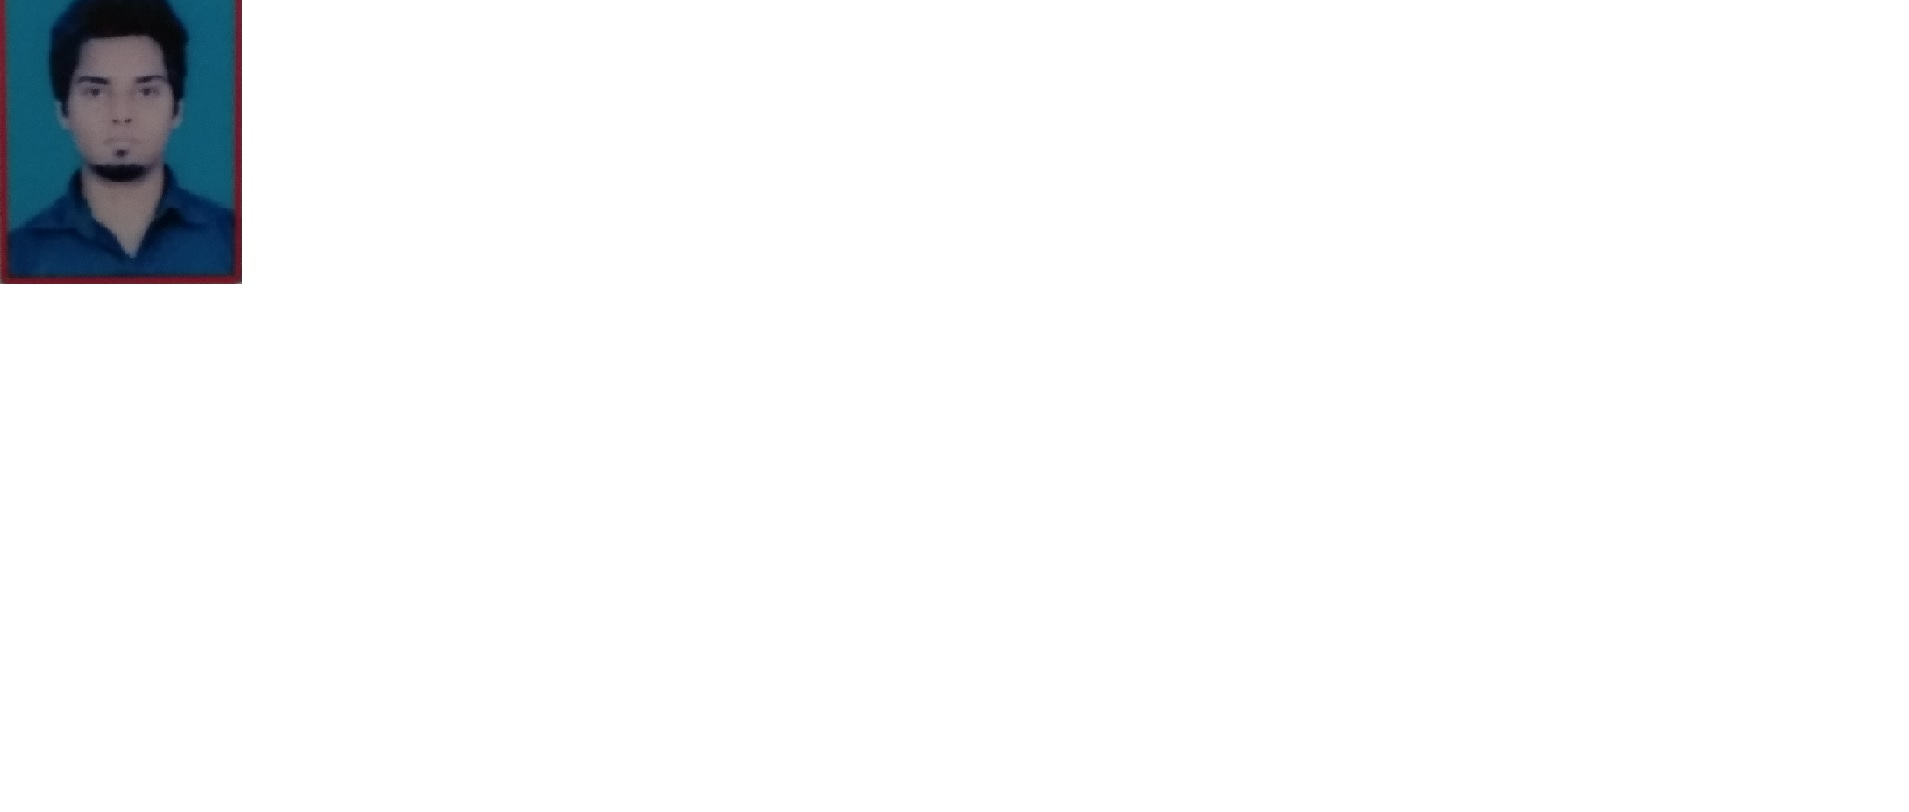
\includegraphics[scale=0.5]{Untitledpic.jpg}} & & \\
%\graphicpath{{C:/Users/VIKRAM/Desktop}}\\
 & &{\huge\bfseries Bikram Keshari Panda} \\
 & & 3rd year
  B.Tech, Electronics \& Telecommunication Engineering \\
 & & VSSUT, Burla \\
 & & Address: Pulaha hall of Residence, VSSUT, Burla\\
 & & email: vikramkeshari002@gmail.com \\
 & & Phone: $+$919439127898 \\
 & &{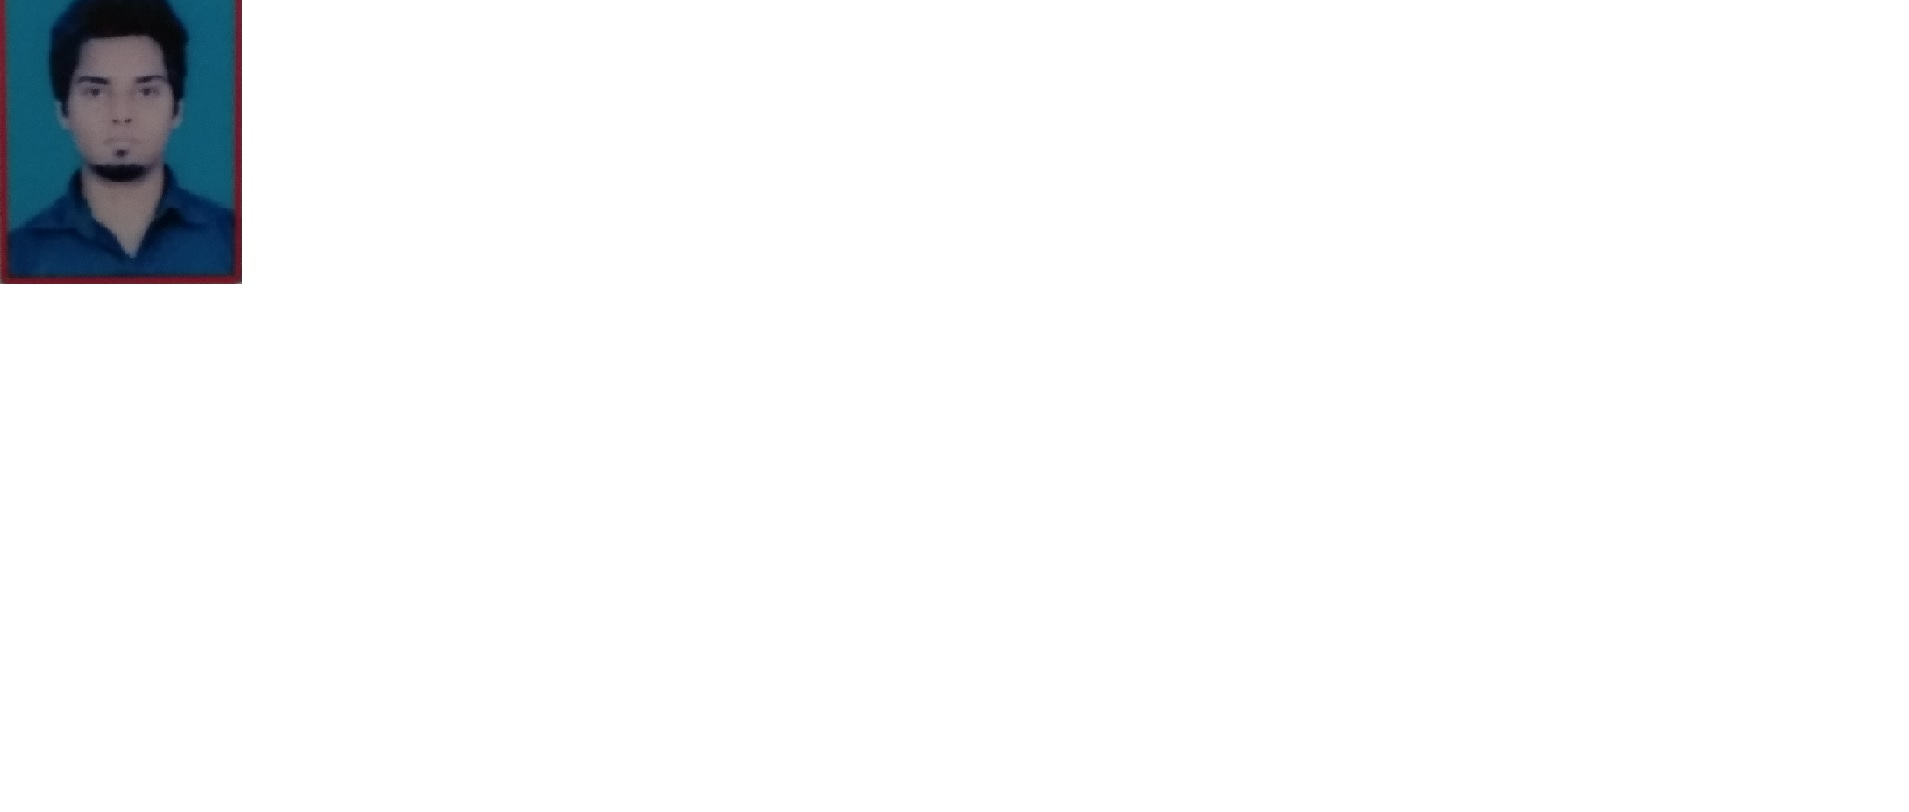
\includegraphics[scale=0.5]{Untitledpic.jpg}} \\
\end{tabular}\vspace{0.5 cm}
%%%%%%%%%%%%%%%%%%%%%%%%%%%%%%%%%%%%%%%%%%%%%%%%%%%%%%%%%%%%%%%%%%%%%%%%%%%%%%%%%%%%%%%%%%
\title{Bikram Keshari-Resume}
\author{Bikram keshari Panda}
\maketitle\vspace{-4 em} \hrulefill
%SIC102,   \hspace{5 in}                                          Contact: 022-2576-4986\\
%ERTS Lab, \hspace{4.8 in}                                 email id: helpdesk@e-Yantra.org\\
%IIT Bombay,Powai,\\
%Mumbai-400076,\\
%Maharastra $
%%%%%%%%%%%%%%%%%%%%%%%%%%%%%%%%%%%%%%%%%%%%%%%%%%%%%%%%%%%%%%%%%%%%%%%%%%%%%%%%%%%%%%%%%%%
\section{ CAREER OBJECTIVE}
 to work in a challenging environment using all my skills and efforts to explore in different fields and seek an opportunity for continuos learning
%%%%%%%%%%%%%%%%%%%%%%%%%%%%%%%%%%%%%%%%%%%%%%%%%%%%%%%%%%%%%%%%%%%%%%%%%%%%%%%%%%%%%%%%%%%
\section{ EDUCATION}
\begin{tabular}{l  p{15 cm}  l}\hline \\
\multirow{3}{*}
{2015-19} &  B-Tech in Electronics \& Telecommunication engineering & \\
 & Veer Surendra Sai University of Technology, Burla & 7.7/10 \\
 & Dist:Sambalpur, Odisha,pin-768018 & \\
 
\\ \multirow{3}{*}
{2014} & 12th(COUNCIL OF HIGHER SECONDARY EDUCATION) & \\
 & Naidu \$+2 Science Recidential College,Bhubaneswar & 80.53\% \\
 & Dist:Khurda, Odisha, pin-760001 & \\ 
 
 \\ \multirow{3}{*}
{2012} & 10th(BOARD OF SECONDARY EDUCATION) & \\
 & Saraswati  Vidya Mandir,Damanjoodi & 91\% \\
 & Dist:Koraput, Odisha, pin-760001 & \\
\\ \hline
\end{tabular}
%%%%%%%%%%%%%%%%%%%%%%%%%%%%%%%%%%%%%%%%%%%%%%%%%%%%%%%%%%%%%%%%%%%%%%%%%%%%%%%%%%%%%%%%%%%%
\section{ Projects}
\begin{tabular}{r  p{15 cm}}
& \begin{itemize} \item Line follower (arduino uno and IR sensor array)
 I was responsible for the design,construction,debugging.\end{itemize}\cr
 
 
 
& \begin{itemize} \item Line follower(using Image Processing)
 I was responsible for the design,construction,PID control,coding(partial),debugging.\end{itemize}\cr
 
  & \begin{itemize} \item Understanding of Data Transmission through OPtical fibre cable and different parameters causing Data loss in it \end{itemize}\cr
 
  & \begin{itemize} \item fuzzzy trafic logic designing and implementation using ARM7 controller\end{itemize}\cr
 
 & \begin{itemize} \item Complete Home Automation using RaspBerry Pi3 and interfacing device in i2c mode\end{itemize}\cr
 
 & \begin{itemize} \item PWM generation with de-bounce circuit and adjustable duty cycle(chip design in verilog HDL)
 I was responsible for the code and debugging.               
\end{itemize}\end{tabular}
\section{TRAINING \& INTERNSHIP }
\begin{itemize}
 \item \textbf{SUMMER VOCATIONAL TRAINING}, Regional Telecom Training Center,BSNL, Bhubaneswar 
 \end{itemize}
\subsection{$\bullet$ \_Training aspects:}
%\subparagraph{•training aspects:} 
%\subsubsection{}
\begin{itemize} \item DIGITAL TRANSMISSION : PCM,PDH,SDH,DWDM,OPTICAL FIBRE CABLE \end{itemize}
 \begin{itemize} \item  DIGITAL SWITCHING AND SUPPORT INFRASTRUCTURE:DSS,POWER PLANT \end{itemize}
 \begin{itemize} \item MOBILE COMMUNICATION:GSM,CDMA,GPRS,EDGE,UMTS(3G),WI-MAX \end{itemize}
  %DATA COMMUNCATION:IPv4,ADSL BROADBAND,NIB,COMPUTER NETWORKING &

%\end{itemize}\cr

 \begin{itemize}
 \item \textbf{SUMMER VOCATIONAL TRAINING} at Central Tool room \& Training Centre for Advanced embedded system with ARM7,PIC,AT89C51.(CTTC),Bhubaneswar.
\end{itemize}




 \begin{itemize}
 \item \textbf{WINTER VOCATIONAL TRAINING} at Embedded technosolutions ,Thane ,Mumbai.
\end{itemize}
\begin{itemize}
 \item \textbf{Personality Development}, Asian Pacific Learning Leverage LTD.
\end{itemize}
%\end{tabular}
\section{RESEARCH PUBLICATION}
None
\section{TECHNICAL SKILLS}
\subsection{languages}
%\subsection{}
\begin{itemize}
 \item \textbf c(experienced)
\end{itemize}
\begin{itemize}
 \item \textbf c++(experienced)
\end{itemize}
\begin{itemize}
 \item \textbf JAVA(experienced)
\end{itemize}
\begin{itemize}
 \item \textbf Python(experienced)
\end{itemize}
\begin{itemize}
 \item \textbf BIOS(beginner)
\end{itemize}
\subsection{Markup languages}
\begin{itemize}
 \item \textbf LaTex(beginner)
\end{itemize}
\begin{itemize}
 \item \textbf HTML(experienced)
\end{itemize}
\begin{itemize}
 \item \textbf BIOCSS(experienced)
\end{itemize}
\section{SOFT SKILLS}
\begin{itemize}
 \item \textbf Quick learner.
\end{itemize}
\begin{itemize}
 \item \textbf Good Analytical skills.
\end{itemize}
\begin{itemize}
 \item \textbf Logical skills.
\end{itemize}
\begin{itemize}
 \item \textbf Initiator and passionate about working.
\end{itemize}
\begin{itemize}
 \item \textbf Good grasping ability.
\end{itemize}
\section{EXTRA-CURRICULAR ACTIVITIES}
\begin{itemize}
 \item \textbf Art and craft.
\end{itemize}
\begin{itemize}
 \item \textbf Painting(professionally trained).
\end{itemize}
\begin{itemize}
 \item \textbf Sports(Badminton,table tennis)
\end{itemize}

\section{CO-CURRICULAR ACTIVITIES}
\begin{itemize}
 \item \textbf National Cadet Corps(N.C.C.)
\end{itemize}
\section{PERSONAL DETAILS}
\subsection{Father's Name}
Mr. Judhisthir Panda
\subsection{Mother's Name}
Mrs. Annapurna Panda
\subsection{Sex}
male
\subsection{date of birth}
13/05/1997
\subsection{Nationality}
Indian
\subsection{Marital Status}
not married
\section{REFERENCE}
\begin{enumerate}
 \item Mr. Aditya Kumar Hota\\
Assistant Professor in Department of Electronics \& Telecommunication Engineering\\
VSSUT, Burla
\item Mr. Bandan Kumar Bhoi\\
Assistant Professor in Department of Electronics \& Telecommunication Engineering\\
VSSUT, Burla
\item Dr. Sanjay Agrawal\\
Associate Professor in Department of Electronics \& Telecommunication Engineering\\
VSSUT, Burla
\end{enumerate}
\section{DECLARATION}
    I,Bikram keshari Panda,hereby declare that all the information mentioned above in this resume are correct to the best of my knowledge. 
\section{Date}
19th April,2018
\end{document} 
